\documentclass[11pt]{article}
\usepackage{aas_macros}
\usepackage{hyperref}
\usepackage{appendix}
\usepackage[hmargin=1.5cm, vmargin=0.55cm]{geometry}
\usepackage{amsmath}
\usepackage{caption}
\usepackage{mathtools}
\usepackage{fancyhdr}
\usepackage{float}%Places the float at precisely the location in the LaTeX code...i.e, [H]
\usepackage{wrapfig}
\usepackage{rotating}
\usepackage{pdfpages}

%for quotes
%\epigraphfontsize{\small\itshape}
%\setlength\epigraphwidth{8cm}
%\setlength\epigraphrule{0pt}


%\usepackage[pdftex]{graphicx}%includegraphics
%converts eps to pdf
\usepackage[update,prepend]{epstopdf}
%\usepackage{subcaption} %need to find subcaption.sty for this to work!
%\usepackage{epstopdf}
\newcommand{\Lagr}{\mathcal{L}}
%\graphicspath{ {~/PhD/Thesis/upgrade-plots/} {./} }
\DeclareGraphicsExtensions{.pdf,.png,.jpg,.eps,.gif,.ps}
\renewcommand{\vec}[1]{\mathbf{#1}}
\usepackage[round]{natbib}  %use the "Natbib" style for the references in the Bibliography
%\usepackage{aastex}%defines journal abbreviations in bib file
%\newcommand{name}[num]{definition}



%\title{Lower Atmospheric Signatures During Solar Flares \\ Associated with Seismicity}
%\author{Jamie Ryan \\
%Mullard Space Science Laboratory \\
%University College London \\
%Surrey, RH13 6NL, UK\\
%\href{mailto:jamie.ryan.14@ucl.ac.uk}{jamie.ryan.14@ucl.ac.uk}
%\date{}}
\begin{document}

\section{Data and Methodology}
%THIS SHOULD DESCRIBE THE SATELLITE DATA AND THE TECHNIQUES USED TO PROCESS AND ANALYSE THESES DATA.
\subsection{Observations and Data Reduction}
Using data collected by spacecraft observing the Sun, energy released during solar flares can be tracked as it is deposited throughout the atmosphere. The X1 flare of the 29th of March 2014 in active region NOAA 12017, was well observed by RHESSI, IRIS and SDO/HMI, collecting HXR, UV and optical emission respectively. The peak of the impulsive phase of the flare occurs at 17:47 UT, at which point all mentioned instruments provide good coverage. The associated sunquake impact is calculated to have area $A_{sqk} \sim 2.6{\times}10^{16}$ $cm^{2}$ and power, $P_{sqk} \sim 1.3\pm0.05{\times}10^{26}$ $erg.s^{-1}$ \citep{2014ApJ...796...85J}.

\subsubsection{The Ramaty High Energy Solar Spectroscopic Imager}\label{rhessi}
%insert RHESSI background info
The Ramaty High Energy Solar Spectroscopic Imager (RHESSI) observes solar emission ranging from 1 keV X-rays to 20MeV $\gamma$-rays produced by energetic particles and nuclear interactions. RHESSI was designed with the aim of understanding impulsive energy release, particle acceleration and transportation in the magnetohydrodynamic environment of the solar atmosphere. Isolating the 10 - 100 keV energy data collected by RHESSI can provide information regarding the intensity and spatial origin of a HXR source. This allows the location of magnetic HXR footpoints to be tracked and the calculation of energy depostion by accelerated electrons. 
  
Practically applying a thick target model fit to RHESSI data is acheived by using the \texttt{ospex} software within SolarSoft (SSWIDL). The entire data set has to be split into short intervals to improve the accuracy of fitting and the detail of resulting plots. The attenuator state of the instrument has to be taken into account due to differences in sensitivity to incoming photons. Therefore it is important to define intervals for fitting first by the attenuator state as \texttt{ospex} will mitigate for the differences in count sensitivity. Then each attenuator time period can be split further in to smaller time increments. 


Shown in Figure \ref{erhessi} is the resulting fit over the impulsive phase of the flare. At the peak of the impulsive phase between 17:46 and 17:48 the RHESSI fit shows an energy ranging from $1.0{\times}10^{28}$ to $2.5{\times}10^{29}$ erg. Assuming the fitting model is correct then the release of this energy is due to non-thermal electrons being accelerated by magnetic reconnection, depositing their energy into the chromosphere. 



\subsubsection{The Interface Region Imaging Spectrograph}
Observing UV ribbons requires a different spacecraft. The Interface Region Spectroscopic Imager (IRIS) captures near-ultraviolet (NUV) and far-ultraviolet (FUV) emission and is designed to observe the chromosphere at various altitudes. Emission is collected by a slit-jaw imager (SJI) and a spectrometer (SG) simultaneously. The spectrograph is sensitive in both FUV and NUV passbands, which expose 3 CCDs to produce spectra in three UV bands, two FUV and one NUV. Table \ref{iris-sg} shows how each passband relates to emission processes occurring from the upper-chromosphere down to the upper-photosphere.

\begin{table}[H]
\centering
\begin{tabular}{|c|c|c|c|}
Band & Wavelength \AA\ & Temperature $\log{T}$ & Region of Atmosphere\\
\hline
FUV 1 & $1331.7 - 1358.4$ & $3.7 - 7.0$ & Upper to lower-chromosphere\\
FUV 2 & $1389.0 - 1407.0$ & $3.7 - 5.2$ & Upper to lower-chromosphere\\
NUV & $2782.7 - 2851.1$ & $3.7 - 4.2$ & Chromosphere to upper-photosphere\\
\end{tabular}
\caption{The IRIS/SG is capable of observing three passbands, which relate to different plasma temperatures.}\label{iris-sg}
\end{table}


The slit-jaw images, are light collected from a reflective area surrounding the slit. The imager is capable of observing four wavelengths relating to emission at different altitudes as shown by Table \ref{iris-sj}.

\begin{table}[H]
\centering
\begin{tabular}{|c|c|c|c|c|}
SJI Passband & Wavelength \AA\ & FWHM \AA\ & Temperature $\log{T}$ & Region of Atmosphere\\
\hline
C II  & $1330$ & $40$ & $3.7 - 7.0$ & Upper-chromosphere\\
Si IV  & $1400$ & $40$ & $3.7 - 5.2$ & Upper-chromosphere\\
Mg II h/k & $2796$ & $4$ & $3.7 - 4.2$ & Lower-chromosphere\\
Mg II wing & $2832$ & $4$ & $3.7 - 3.8$ & Upper-photosphere\\
\end{tabular}
\caption{The IRIS/SJ is capable of observing four passbands, which relate to different plasma temperatures.}\label{iris-sj}
\end{table}


The IRIS spacecraft captured the temporal evolution of the flare between 14:09 and 17:54 UT via it's slit-jaw imager and spectrograph at solar coordinates 491", 282", with a spatial resolution of 0.1667" per pixel. The slit-jaw imager data provides coverage of a field of view spanning 167" by 174", of passbands that including 1403, 2796 and 2832 \AA\ at 26, 19 and 75 second cadence respectively. The spectrograph slit has a field of view spanning 14" by 174" and is aligned directly over chromospheric flare ribbons, and the sunquake point of origin. For the majority of the observation, the spectrograph slit is exposed for $\sim9$ seconds at 8 slit locations for a total of 72 seconds cadence per raster. However, during the impulsive phase the IRIS SG shortens it's exposure time to around 2.4 seconds in order to mitigate against saturation of the CCDs. Wavelengths observed over three channels include FUV1: 1331.7 - 1358.4 \AA, FUV2: 1389.0 - 1407.0 \AA\ and NUV: 2782.7 - 2851.1 \AA, associated with the transition region, chromosphere and the upper-photosphere. Spectral lines include C II, Si IV and Mg II h and k. IRIS SJI data is the standard level 2 data product provided for scientific research, which has been calibrated to negate dark currents, flat-field and spacecraft rotational effects. In order to observe flare ribbons in the photospheric data captured by IRIS SJI MG II wing channel, a running difference filter is applyed. This effectively removes unwanted background features, highlighting the UV ribbons. IRIS SG data is manually corrected for changing exposure times and wavelength shifts caused by the orbital motions of the spacecraft. IRIS SG data is sampled over a wavelength range of 2825.7 and 2825.8\AA\ which represents a sample of Balmer pseudo-continuum. 

The next stage of the processing requires that IRIS SJ and SG data are converted from relative intensity (DN per pixel) to energy (erg) units. This is acheived by using a method provided in the instrument documentation \citep{2014SoPh..289.2733D} which calculates the conversion factors between relative DN.s$^{-1}$ units and absolute erg.s$^{-1}$.cm$^{-2}$.sr$^{-1}$.\AA\ $^{-1}$ units via equation \ref{irisradiometriccal}. Where $I_{dn}$ is relative intensity in units of DN per pixel, $C_{d2p}$ is the DN to photon conversion factor provided by \cite{2014SoPh..289.2733D}, $E_{\lambda}$ is the photon energy, $A_{eff}$ is the effective area, $t_{exp}$ is the exposure time, $d_{\lambda}$ is the wavelength dispersion, $\Omega$ is the solid angle and $I_{abs}$ is the intensity in absolute units.

\begin{equation}\label{irisradiometriccal}
I_{abs} = \frac{{I_{dn}} \; {C_{d2p}} \; {E_{\lambda}}}{{A_{eff}} \; {t_{exp}} \; {d_{\lambda}} \; {\Omega}}
\end{equation}
%    fout = (array*n_pixels*dn2photon*E_photon)/(A_float*texp*pixlambda*w) ;erg/s.cm^2.sr.Å



\subsubsection{The Solar Dynamics Observatorie's Helioseimic and Magnetic Imager}
Signatures of energy deposition in the lowest regions of atmosphere are captured by Solar Dynamics Observatory's (SDO) Helioseismic Imager (HMI), which is sensitive to the wing of the photospheric absorption line 6173 \AA\ (Fe I), which is essentially optical continuum. SDO/HMI has three main observables, continuum, dopplergrams and magnetic field configuration, each of which can provide valuable insight into the physical conditions existing in photospheric plasma. In particular for this project, optical continuum data can provide information about WLFs intensity, which along with Balmer continuum could be linked to radiative backwarming of photospheric material, which is a possible sunquake progenitor. The point of origin and wave-fronts of the sunquake can also be detected using helioseismic data, which can be used to calculate acoustic power of the quake.
The HMI instrument onboard SDO observes the entire solar photosphere with 4k resolution and a pixel size relating to 0.505" by 0.505", with each image having a cadence of 45 seconds. The data is calibrated to negate cosmic-rays, dark currents, flat-field and spacecraft rotational effects. In this project, HMI continuum data is used primarily to observe White light flares, which are difficult to see against the bright photospheric background. To highlight the positions of flare ribbons in the photosphere, data must be filtered. Silimarly to \cite{2014ApJ...783...98K}, photospheric continuum data captured by HMI is put through a two stage filtering porcedure. First the data has an unsharp filter applied, so that the filtered image, $I_{filt}=I-$ smooth($I$,10), where $I$ is the original image and the function smooth relates to a 10 pixel boxcar smoothing filter, this is to remove small features such as granulation. The technique is not perfect meaning that some granulation is still visible after the unsharp filter. Second, $I_{filt}$ is subjected to a running difference filter to isolate locations that are white-light enhanced. The running difference filter effectively removes static features leaving behind those pixels that are changing over short time-scales. However, for removing signatures of those processes occurring over shorter time periods such as the remaining granulation and also p-mode oscillations, this filtering technique is ineffective. This is not a problem, as for the purpose of white light flare analysis, the data yield a strong contrast between flare-enhanced and background pixels after being filtered by a $i-2$ running difference. The next stage is to determine which pixels in the difference image are those that are enhanced during the flare. For the best result, white-light enhanced pixels are identified using a combination of visual inspection and thresholding. Attempts at automating the identification process tend to lead to false positives being triggered by noise or granulation features. \\
HMI Dopplergrams are used in conjunction with holography techniques to produce a 6mHZ acoustic egression power map (supplied via private communication by Sergei Zharkov) revealing the location of the sunquake. 

As with the IRIS data, the next stage of processing is to convert relative intensity into absolute intensity. To perform this conversion for SDO HMI data the basic equation \ref{irisradiometriccal} is used with values tailored for HMI. A combination of sources \citep{2012SoPh..275...41B, 2012SoPh..275..285C} have been used to find the instrument's properties which are used to fulfil a conversion factor. Where $g$ is the instrument gain, $QE$ is the quantum efficiency of the charged couple device and $r_{ap}$ is the instrument aperture radius, $\Upsilon$ is the relative filter assembly transmittance and all other terms are the same as equation \ref{irisradiometriccal}.


\begin{equation}\label{hmiradiometriccal}
I_{abs} = \frac{I_{dn} \; C_{d2p} \; E_{\lambda}}{A_{eff} \; t_{exp} \; d_{\lambda} \; \Omega} 
        = \frac{I_{dn} \; g \; QE \; E_{\lambda}}{\pi \; r_{ap}^{2} \; \Upsilon \; t_{exp} \; d_{\lambda} \; \Omega} 
\end{equation}


\subsection{Data Sampling}
For the IRIS SJI, IRIS SG and SDO HMI data sets, multiple sample points have been chosen based on the moment in time when the IRIS SG slit is directly over the southern flare ribbon and sunquake impact location. These coordinates are sampled across all data sets except RHESSI. Figure \ref{hmicontext} shows the sample coordinates, RHESSI HXR and the 6mHz sunquake egression map, plotted over filtered SDO HMI data in an effort to demonstrate the spatial alignment between HXR (particle beam), UV ribbons and sunquake impact. Table \ref{coordtab} shows how each sample number relates to a heliocentric position in arcseconds.


\begin{table}[h]

\begin{tabular}{|c|c|}
\hline
Sample Number & Heliocentric Position (x,y)\\
\hline
1 & 518.219", 262.000"\\
2 & 520.215", 263.000"\\
3 & 522.212", 262.000"\\
4 & 522.212", 265.000"\\
5 & 524.256", 265.000"\\
6 & 526.252", 263.818"\\
\hline
\end{tabular}
\caption{Sample number and the corresponding coordinates in heliocentric units (arcsec).}\label{coordtab}
\end{table}

%need to run hmi_context_plot.pro
\begin{figure}[H]
  \begin{center}
  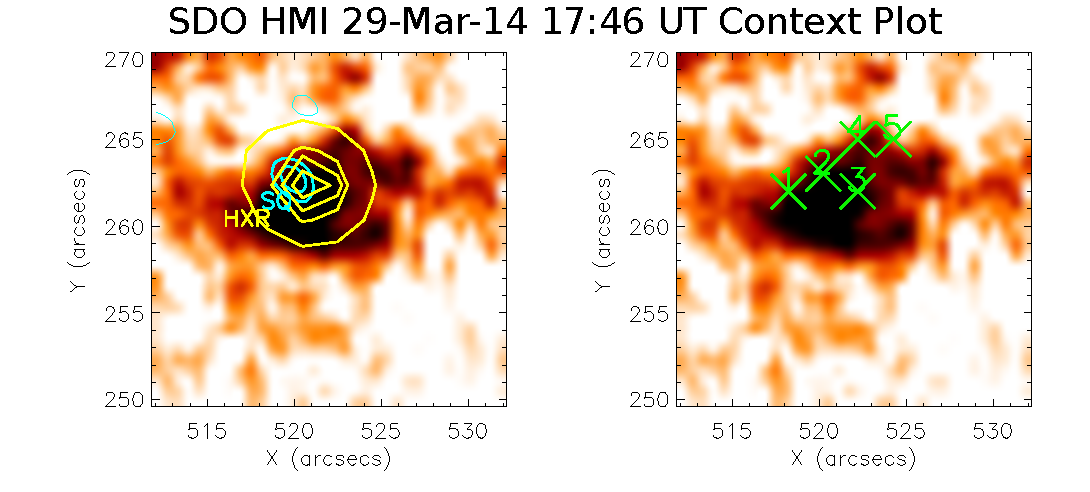
\includegraphics[width=0.8\textwidth]{29-Mar-14-HMI-Sunquake-Context-Plot}
  \end{center}
  \caption{The images show SDO HMI continuum data in reverse colour scheme; with the left image displayng yellow contours representing 50 to 100 keV HXR emission at 80, 90, 92, 94, 96 and 98$\%$ of maximum and 6mHz sunquake power in cyan; the right image shows sample coordinates as green crosses with their associated number relating to Table \ref{coordtab}. Each of the IRIS SJ, IRIS SG and SDO HMI data sets are sampled at the exact same coordinates in heliocentric units.}\label{hmicontext}
\end{figure}


\section{Results and Discussion}
\subsection{RHESSI Hard X-rays}
%RHESSI
For a sunquake to be generated by accelerated paticle collision then the incident beam must be aligned over the acoustic impact location \citep{1998IAUS..185..191K}. To highlight this spatial alignment, RHESSI 50 to 100 keV HXR and sunquake egression power contours are plotted on a reverse colour, filtered HMI continuum image shown in figure \ref{hmicontext}. The contours show a reasonable alignment but a more rigorous way to test the spatial and temporal relationship between HXR, sunquake and other emission is to analyse lightcurves from the region of interest.   %explain alignment of different faetures and the significance      

RHESSI HXR data is taken from central coordinates 518" by 262", sampling the sunquake epicenter. When this data is fit to a nonthermal electron model a spectrum is produced, which can be used to plot the energy curve shown in Figure \ref{erhessi}. The plot shows 10 - 100 keV HXR power as a function of time. The impulsive phase of the flare is visible from 17:46, peaking at 17:47, with the plot showing a double peak profile which climbs from $1.0{\times}10^{28}$ to $2.5{\times}10^{29}$ erg. To put this in the context of the associated sunquake, the HXR energy can be used to estimate the amount of energy provided to the acoustic impact area, or nonthermal flux via

\begin{equation}\label{electronflux}
F_e = \frac{P_{e}}{A_{HXR}}
\end{equation}

where flux $F_e$ is in units of erg.s$^{-1}$.cm$^{-2}$, $P_e$ is nonthermal power and the HXR emission area is determined by the $90\%$ HXR contour in Figure \ref{hmicontext}, rendering $A_{HXR} \sim \pi (2"{\times}7.25{\times}10^{7})^{2} = $ cm$^{2}$. The resulting flux turns out to be $F_e \sim 10^{44}$ which when multiplied

can be multiplied by the sunquake area, to determine an upper limit for the nonthermal power available for generating an acoustic disturbance $P_{e}(A_{sqk}) = \frac{F_e}{A_{sqk}}$. So using 10\% of the available nonthermal energy, $P_e \sim 10^{28}$ erg.s$^{-1}$cto cater for the fact that only emission of $90\%$ and above maximum, and $A_{sqk} \sim 2.6{\times}10^{16}$ $cm^{2}$. $P_{e}(A_{sqk}) \sim 10^{28}$ and when compared with the sunquake power $P_{sqk} \sim 1.3\pm0.05{\times}10^{26}$ $erg.s^{-1}$ it is clear that the electron beam does have the required 1000 times more energy required to the sunquake. Another interesting quantity to investigate is the momentum of the particle beam. Electron momentum can be calculated by 


\begin{equation}\label{electron-momentum}
p_e=\tau \sqrt{2m_e} P_{e}
\end{equation}

where $m_e$ is electron mass, $\tau$ is the time duration of flare impulsive phase and $P_{e}$ is described by equation \ref{pnth1}. Substituting values in to equation \ref{electron-momentum} yields an electron momentum of $p_e \sim 1.35{\times}10^{17}$ g cm s$^{-1}$. Assuming the energy in the electron beam is equal to that in a population of accelerated protons, then calculation of a theoretical proton beam momentum, where $m_p$ is the proton mass, is by the relation,

\begin{equation}\label{proton-momentum}
p_p \sim p_e \sqrt{\frac{m_p}{m_e}}
\end{equation}

Which yields a proton momentum of $p_p \sim 5.79{\times}10^18$ g cm s$^{-1}$, an order of magnitude greater than $p_e$. This is because $m_p ~ 2000m_e$ meaning the square root in equation \ref{proton-momentum} renders the result $p_p \sim 44.7p_e$. So in order to determine whether a particle beam carries enough momentum to stimulate a sunquake, a calculation of the momentum needed to initiated the acoustic response is required.\\

The momentum needed to produce the sunquake is

\begin{equation}
p_{sqk}\sim \rho \; l^{3} \; v
\end{equation}\label{sqk-momentum} 

where all terms are tailored for photospheric values, hence density $\rho \sim 10{-8}$g cm$^{-3}$; sound speed $v \sim 10^{6}$ cm.s$^{-1}$. The length-scale, $l \sim  1.82{\times}10_{8}$, corresponds to the sunquake impact diameter, 

\begin{equation}
l = 2\sqrt{\frac{A_{sqk}}{\pi}}
\end{equation}\label{lengthscale}

Equation \ref{sqk-momentum} gives the momentum of the acoustic reponse as $p_{sqk} = 6.03{\times}10^{22}$ g cm s$_{-1}$, which when compared to particle beam momenta, $p_e$ and $p_p$, is $10{5}$ and $10^{4}$ times larger respectively. This means that even if an electron or proton beam can make it down to the photosphere, it wouldn't have the necessary momentum to cause the sunquake on it's own. In reality, calculated momenta are idealistic, not treating the effects of energy loss due to energy dissapation. The point being that for a particle beam to make it to the photosphere, it has to traverse 9 pressure scale heights, increasing in density with depth. As density increases particles in the beam are more likely to encounter ambient plasma, and as a result are deccelerated, giving up as energy as emission. So if or when the beam reaches the photosphere, much of it's energy and momentum has already been dissapated in the chromosphere, making the generation of a sunquake via just the particle beam even more unlikely.

\begin{figure}[H]
  \begin{center}
  \textbf{RHESSI 10 - 100 keV Hard Xray Energy Over Time}\par\medskip
  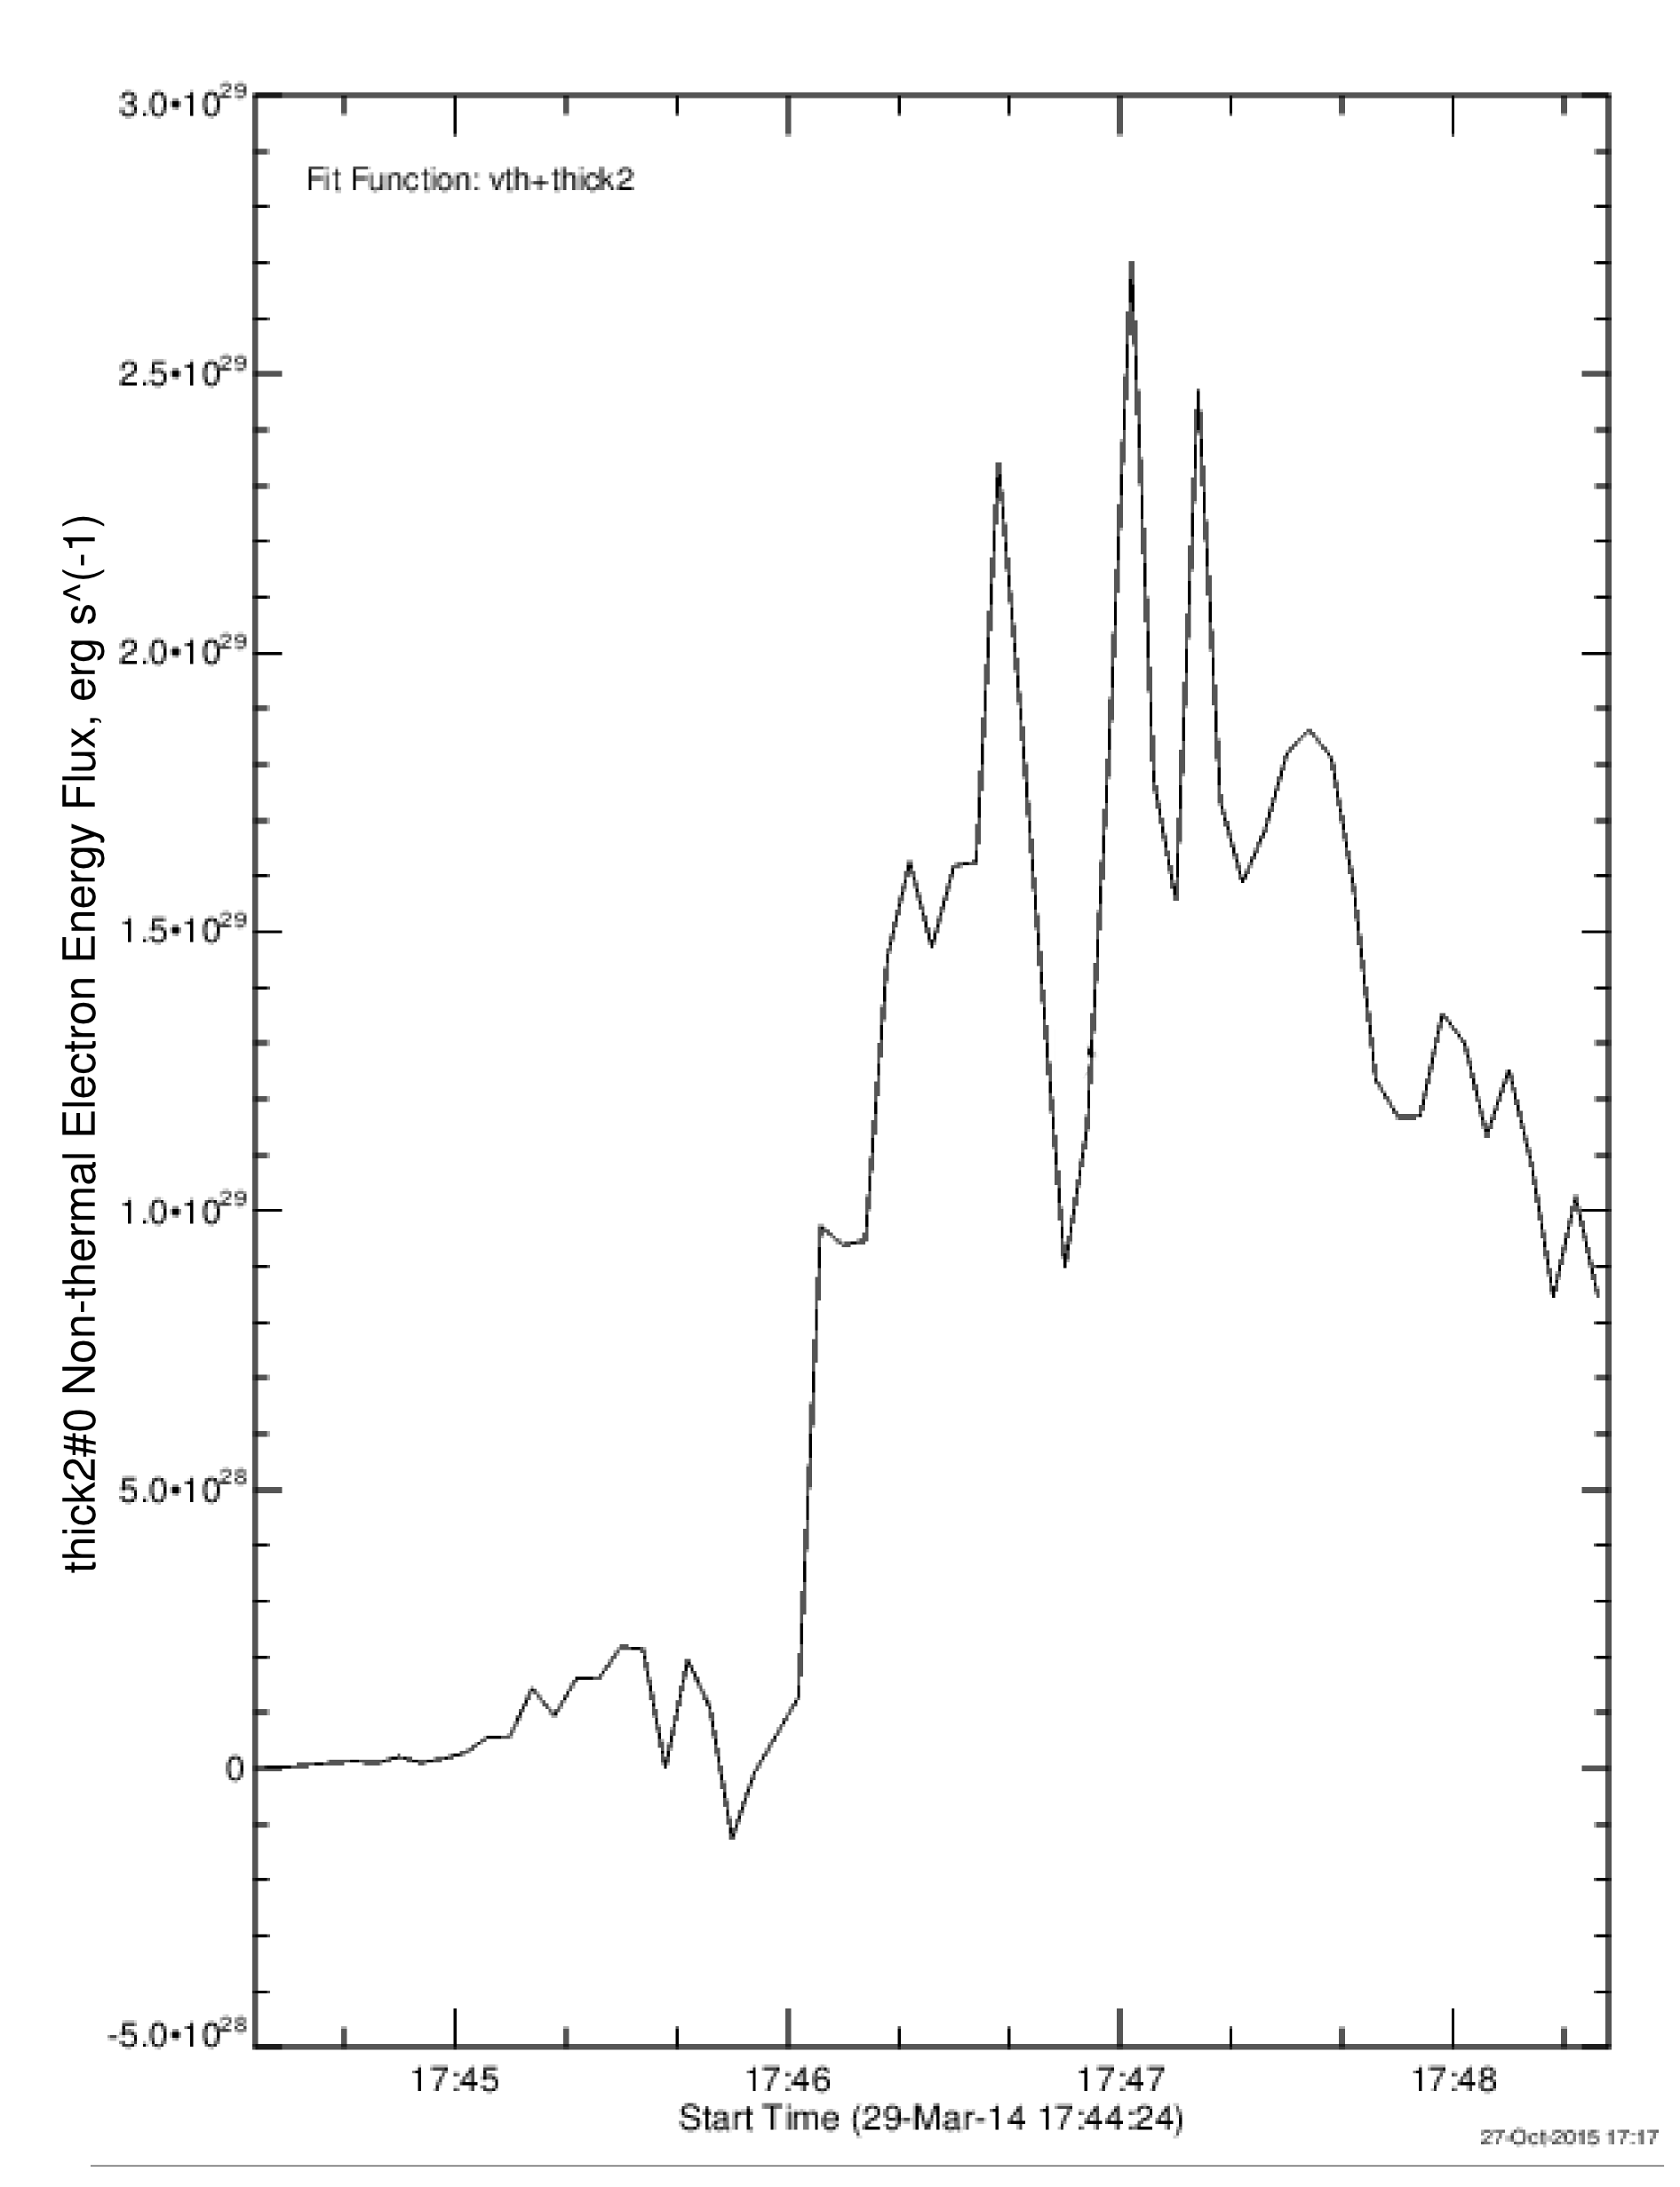
\includegraphics[width=0.6\textwidth]{rhessi-energy-curve}
  \end{center}
  \caption{Shows the energy evolution of hard x-ray emission collected by RHESSI 10 to 100 keV bins over the sunquake region (518", 262"). HXR emission is due to non-thermal electrons, thus energy is calculated by fitting data to the collisional thick target model. The HXRs impulsive phase begins at around 17:46 and peaks at 17:47, showing temporal alignment with IRIS and HMI datasets shown if Figure \ref{fluxladder}}
\end{figure}\label{erhessi}

\subsection{Emission Captured By IRIS and HMI}
%Si IV, Mg II, Balmer, MG II w, HMI
However, energy deposited into the atmosphere by the particle beam can lead to other sunquake generation mechanisms, such as radiative backwarming and shocks which are described in sections \ref{sunprog}. A recent result from \cite{2016ApJ...816...88K} shows that the intensity of Balmer continuum observed in this event could come from either; 23\% of nonthermal electrons with energy $<20$ keV; or the entire population of nomthermal electrons with energy $<40$ keV. This means that a large portion of energy delivered to the lower atmosphere by the electron beam is dissapated causing various continua and emission lines. Shown in Figure \ref{fluxladder} are lightcurves of emission from the lower solar atmosphere, captured by IRIS and SDO HMI. From top to bottom the plot shows data from IRIS SJ Si IV, IRIS SJ Mg II, IRIS SG Balmer Continuum, IRIS SJ Mg II wing and SDO HMI visible continuum sampled from six coordinates in the flare ribbon. Si IV and Mg II IRIS SJ data, show a distinct cutoff which is caused by over saturation of the instrument CCD, meaning flux measurements during the impulsive phase are a lower estimate. However, Si IV and Mg II lightcurves can still be used to confirm temporal and spatial alignment of energy deposition at these wavelengths. All coordinates in all datasets show a synchronised impulsive peak, with the exception of MG II wing where only coordinates four and five exhibit a siginifcant enhancement. The red solid line in each data set is sampled from the sunquake location. At first glance the sunquake location in the plots does not seem to have any obvious differences other than a slight time delay in peak Balmer continuum emission. The delay appears to be around 45 seconds after the impulsive phase peak at approximately 17:48 which coincides with the sunquake onset time \citep{2015ApJ...812...35M}. Mg II wing data shows no enhancement over the sunquake location. HMI continuum shows significant enhancement over the sunquake, which is aligned in time with the impulsive phase. 




%LADDER PLOTS
\begin{figure}[H]
  \begin{center}
  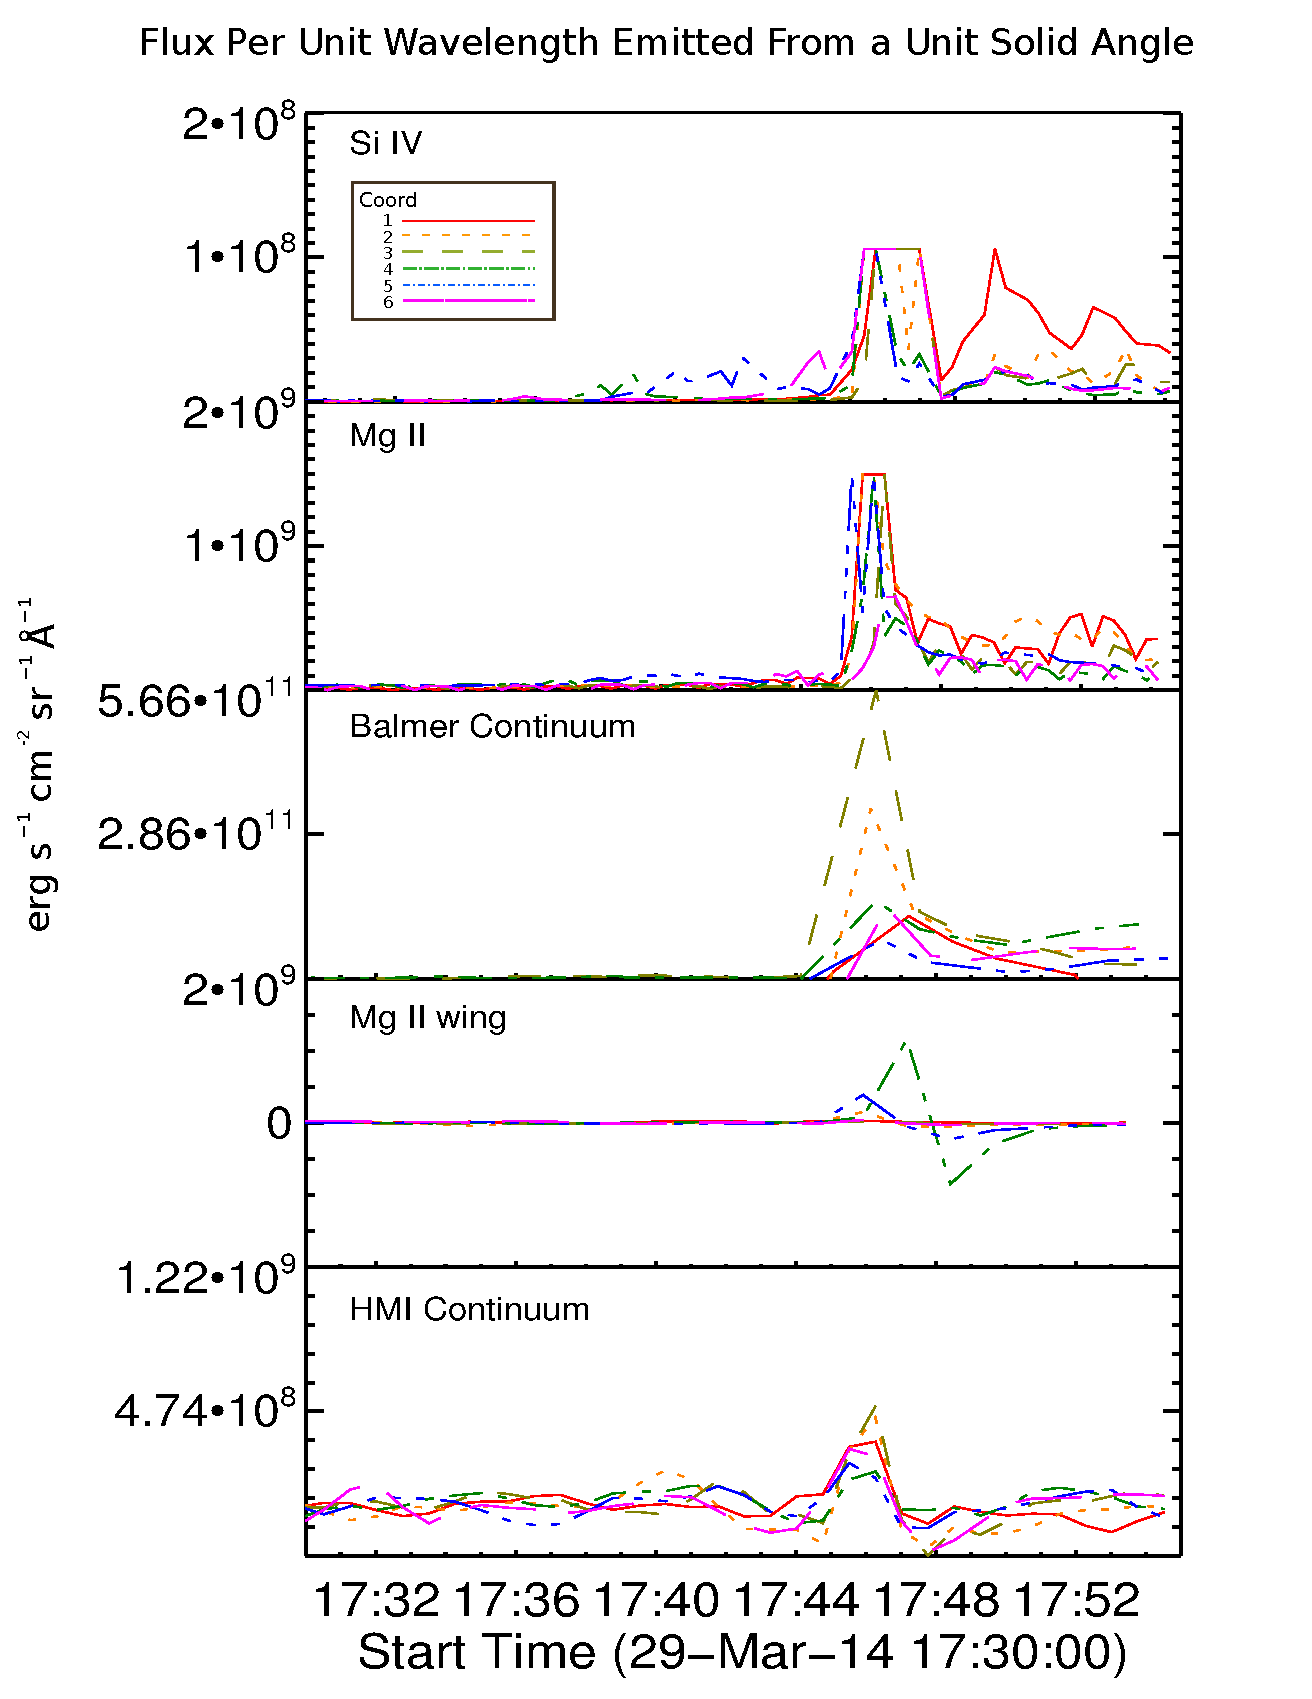
\includegraphics[width=0.6\textwidth]{29-Mar-14-Flux-Ladder}
  \end{center}
  \caption{Shows flux per wavelength from a unit solid angle or intensity. The six lines (see legend) represent areas centered on regions 1 to 6, relating to heliocentric coordinates shown in Table \ref{coordtab}. The solid red line is directly over the sunquake location. Each plot represents an independant data set, in order from top to bottom the sets are; IRIS SJ 1400 (Si IV); IRIS SJ 2796 (Mg II); IRIS SG  2825.7 to 2825.8 (Balmer Continuum); IRIS SJ 2832 (Mg II wing); SDO HMI continuum}\label{fluxladder}
\end{figure}




\begin{figure}[H]
  \begin{center}
  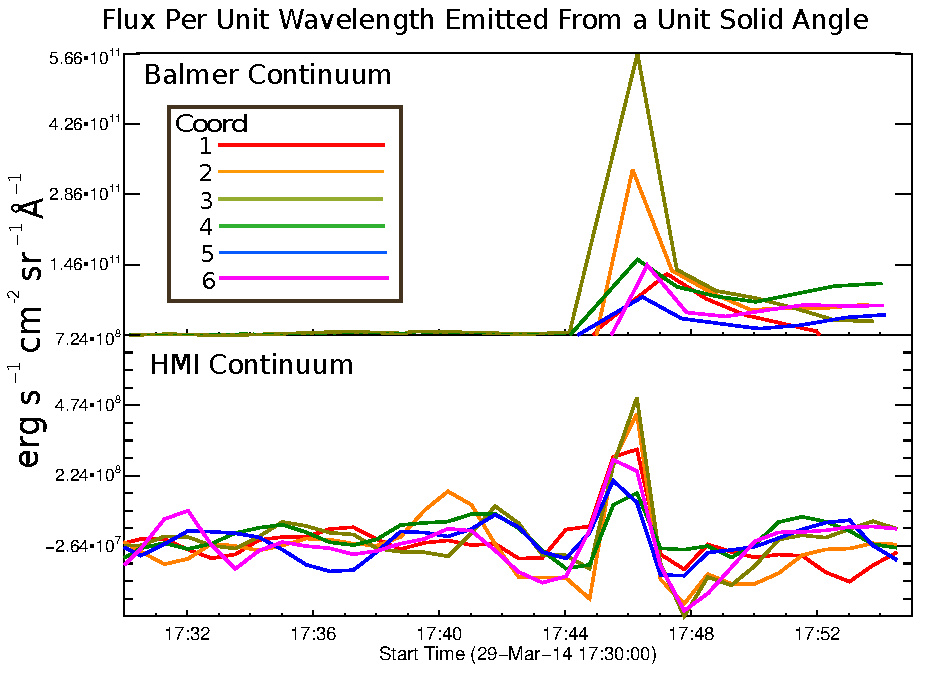
\includegraphics[width=0.6\textwidth]{29-Mar-14-Flux-Ladder-Balm-HMI-Only}
  \end{center}
  \caption{Shows flux per wavelength from a unit solid angle. The six lines (see legend) represent areas centered on regions 1 to 6, relating to heliocentric coordinates shown in Table \ref{coordtab}. The solid red line is directly over the sunquake location. Each plot represents an independant data set, in order from top to bottom the sets are; IRIS SJ 1400 (Si IV); IRIS SJ 2796 (Mg II); IRIS SG  2825.7 to 2825.8 (Balmer Continuum); IRIS SJ 2832 (Mg II wing); SDO HMI continuum}\label{fluxladder-balm-hmi-only}
\end{figure}


The flux values for Balmer and HMI continuum shown in Figure \ref{fluxladder-balm-hmi-only} can be used to estimate the power of the radiative backwarming. The key being whether the radiative backwarming is powerful enough to generate the white light flare and hence the sunquake. The power profiles shown in Figure \ref{powerladder-balm-hmi-only} are calculated by assuming a homogenous energy distribution in the region surrounding each coordinate, it is then possible to use the relation,

\begin{equation}
P_{Balm} = F_{Balm} \; A_{sqk}  
\end{equation}\label{Pbalm}

where $P_{Balm}$ is the power of the Balmer continuum emitted from an area equal to the sunquake, $A_{sqk}$. The same data set and coordinate scheme is followed as in Figure \ref{fluxladder-balm-hmi-only}. The Balmer continuum over the sunquake shows an impulsive power $P_{Balm} = 6{\times}10^{13}$ erg.s$^{-1}$ which is thirteen orders of magnitude smaller than the power of the sunquake $P_{sqk} \sim 1.3\pm0.05{\times}10^{26}$ $erg.s^{-1}$. This means that there is not enough energy per second deposited by radiative backwarming to create the sunquake. The HMI continuum power, $P_{HMI}$, over the sunquake location peaks at $P_{HMI} = 2{\times}10^{14}$ erg.s$^{-1}$cm$^{-2}$, which is twelve orders of magnitude less than the $P_{sqk}$ but ten times greater than the Balmer continuum. One of the biproducts of radiative backwarming are white light flares in the photosphere. Balmer continuum radiated outward to the observer, is supposed to be equal in power to that emitted downward \citep{1989SoPh..124..303M}. In that case the white light flare shown in the HMI continuum in Figure \ref{powerladder-balm-hmi-only} is only provided $10\%$ of its power by radiatve backwarming. So radiative backwarming at first glance may not be causing the observed white light emission. However, another way to investigate the energy deposition in the lower atmosphere is by integrating radiative flux over the impulsive phase of the flare. This provides an upper limit for the total flux injected into the system during the impulsive phase, which can be used to calculate the total emission power. The integrated flux is calculated,

\begin{equation}
F_{imp} = \int_{0}^{\tau} F(t) \; dt = F(t) \; \tau
\end{equation}\label{f-imp}
 
where the duration of the impulsive phase $\tau = $ and $F(t)$ is the emitted flux at time $t$. The total power emitted during the impulsive phase, $F_{imp}$ is

\begin{equation}
P_{imp}=F_{imp} \; A_{sqk}
\end{equation}\label{e-imp}

where it is assumed that a homogenous energy distribution exists throughout the sunquake impact area. This produces values for each data set tabulated in Table \ref{eimp}. Balmer and HMI continua are the data sets that show the highest integrated energy levels, with comparable values at each coordinate. The fact that Balmer and HMI continua show such similar energies emitted over the impulsive phase means that radiative backwarming is likely causing the white light flare in the photosphere as described in section \ref{wlf}. The highest energy reading in the HMI continuum is over the sunquake, with a value of $1.42{\times}10^{16}$ erg whereas in the Balmer continuum the highest is coordinate three with $2.52{\times}10^{16}$, both of which are ten orders of magnitude smaller than $P_{sqk}$. Meaning that the radiative backwarming mechanism in this case is not powerful enough to produce the sunquake.    


%\begin{figure}[H]
%  \begin{center}
%  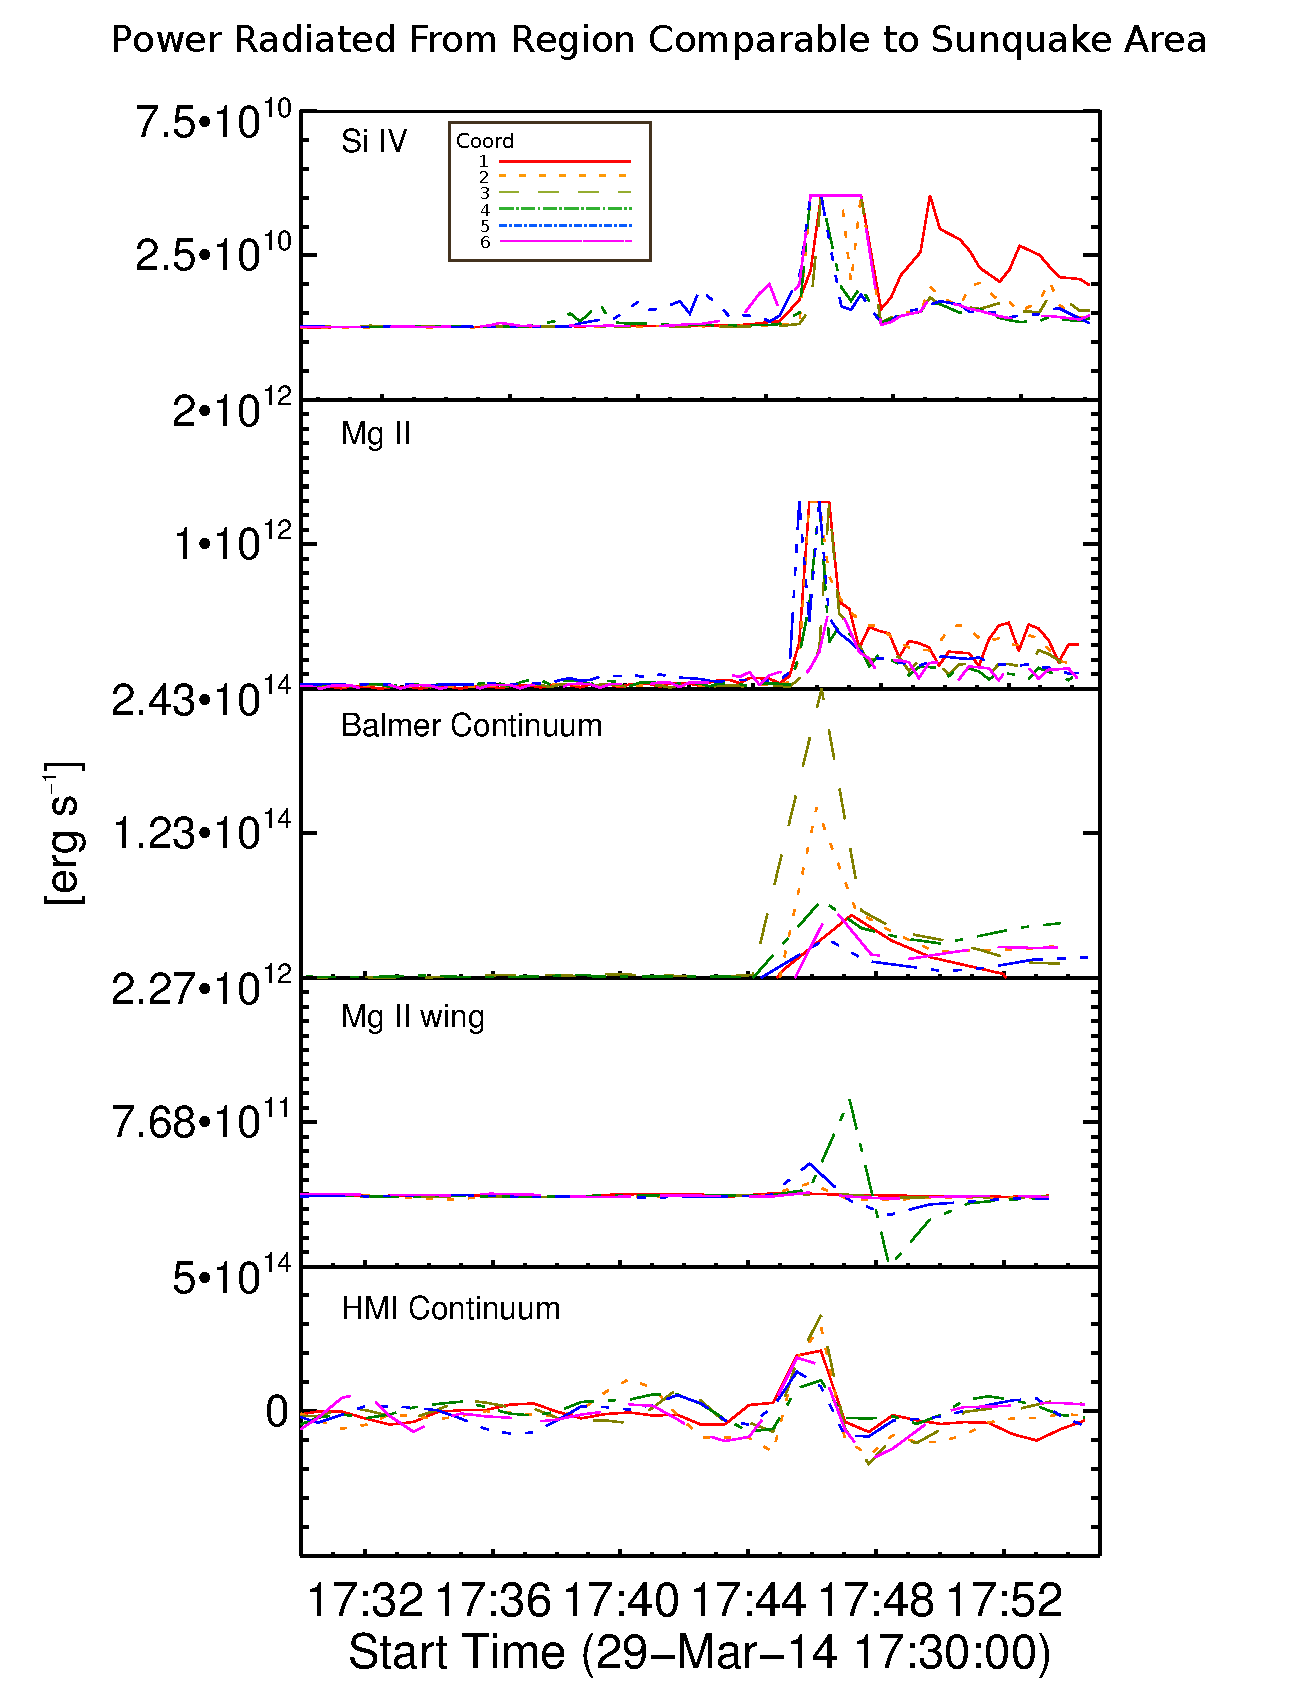
\includegraphics[width=0.6\textwidth]{29-Mar-14-A_sqk-Power-Ladder}
%  \end{center}                                                                                                                                                                                                                                                                                                                                                                                                                                                                                                                                                                                                                                                                                                                                                                                                                                                                                                                                                                                                                                                                                                                                                                                                                                                                                                                                                                                                                                                                                                                                                                                                                                                                                                                                                                                                                                                                                                                                                                                                                                                                                                                                                                                                                                                                                                                                                                                                                                                                                  
%  \caption{Shows radiative power [erg.s$_{-1}$], which is the result of flux data that has been multiplied by the sunquake impact area. The six lines (see legend) represent areas centered on regions 1 to 6, relating to heliocentric coordinates shown in Table \ref{coordtab}. The solid red line is directly over the sunquake location. Each plot represents an independant data set, in order from top to bottom the sets are; IRIS SJ 1400 (Si IV); IRIS SJ 2796 (Mg II); IRIS SG  2825.7 to 2825.8 (Balmer Continuum); IRIS SJ 2832 (Mg II wing); SDO HMI continuum (HMI).}\label{powerladder}
%\end{figure}

\begin{figure}[H]
  \begin{center}
  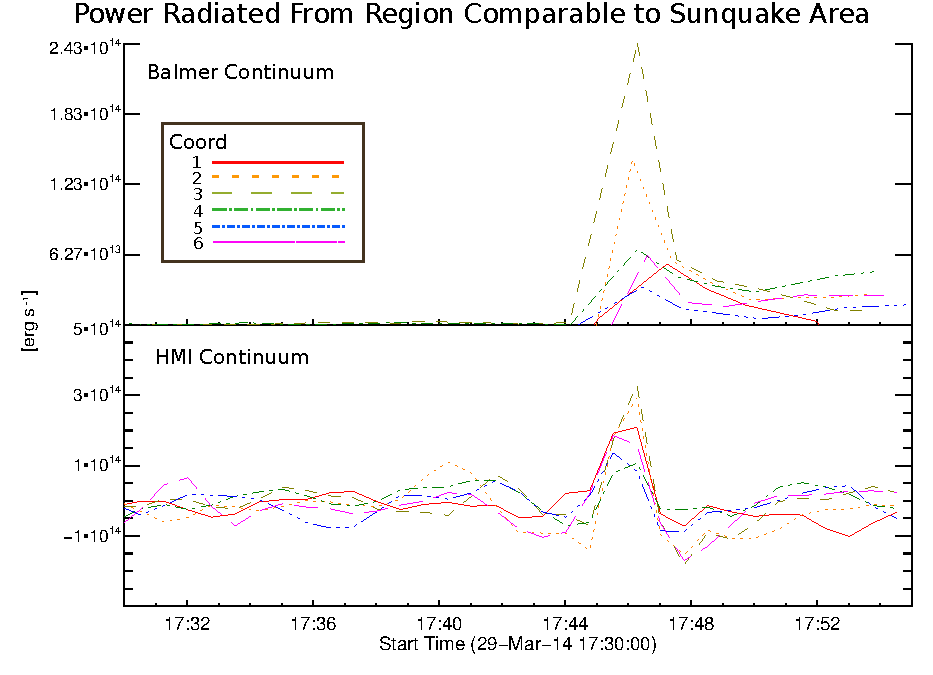
\includegraphics[width=0.6\textwidth]{29-Mar-14-A_sqk-Power-Ladder-Balm-HMI-Only}
  \end{center}
  \caption{Shows radiative power [erg.s$_{-1}$], which is the result of flux data that has been multiplied by the sunquake impact area. The six lines (see legend) represent areas centered on regions 1 to 6, relating to heliocentric coordinates shown in Table \ref{coordtab}. The solid red line is directly over the sunquake location. The top plot is IRIS SG  2825.7 to 2825.8 Balmer Continuum and the bottom plot is SDO HMI continuum.}\label{powerladder-balm-hmi-only}
\end{figure}




\begin{table}[h]
%\tiny
\centering
\begin{tabular}{|c|c|c|c|c|c|c|c|c|c|c|}
Coord Number & Coorinates (x,y) [arcsecs] & $E_{Si IV}$ [erg] & $E_{Mg II}$ [erg] & $E_{Balm}$ [erg] & $E_{Mg II w}$ [erg] & $E_{HMI}$ [erg]\\
\hline
1 & 518.22, 262.00 & 6.74E+12 & 1.41E+14 & 5.98E+15 & 4.27E+12 & 1.42E+16\\
2 & 520.22, 263.00 & 5.65E+12 & 1.35E+14 & 1.71E+16 & 7.14E+12 & 1.10E+15\\
3 & 522.21, 262.00 & 5.18E+12 & 7.83E+13 & 2.52E+16 & 2.91E+12 & 4.82E+15\\
4 & 522.21, 265.00 & 3.93E+12 & 8.35E+13 & 9.89E+15 & 6.70E+13 & 1.28E+15\\
5 & 524.26, 265.00 & 3.98E+12 & 1.03E+14 & 4.37E+15 & 1.86E+13 & 8.99E+14\\
6 & 526.25, 263.82 & 6.91E+12 & 6.34E+13 & 5.24E+15 & 1.74E+12 & 9.88E+14\\
\end{tabular}
\caption{Flux integrated over the flare impulsive phase (17:44 to 17:48) is then multiplied by the sunquake impact area to produce a total deposited energy in erg. The values show are for ribbon sample locations 1 to 6.}\label{eimp}
\end{table}







\label{Bibliography}
\lhead{\emph{Bibliography}}  % Change the left side page header to "Bibliography"
%\bibliographystyle{unsrtnat}  % Use the "unsrtnat" BibTeX style for formatting the Bibliography
\bibliographystyle{plainnat}%abbrv}
\bibliography{../Bibliography/Bibliography}  % The references (bibliography) information are stored in the file named "Bibliography.bib"
%\bibliography{Bibliography}
\end{document}
